\documentclass[12pt,a4paper]{article}
\usepackage{tikz}
\begin{document}

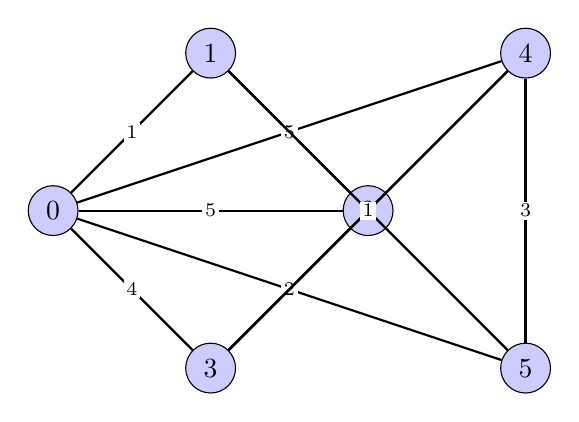
\begin{tikzpicture}[
    vertex/.style={circle, draw, fill=blue!20, inner sep=2pt, minimum size=18pt},
    edge/.style={draw, thick},
    weight/.style={font=\scriptsize, midway, fill=white, inner sep=1pt}
]

% Define vertices
\node[vertex] (0) at (0, 0) {0};
\node[vertex] (1) at (2, 2) {1};
\node[vertex] (2) at (4, 0) {2};
\node[vertex] (3) at (2, -2) {3};
\node[vertex] (4) at (6, 2) {4};
\node[vertex] (5) at (6, -2) {5};

% Define edges with weights
\path[edge] (0) -- node[weight] {1} (1);
\path[edge] (0) -- node[weight] {5} (2);
\path[edge] (0) -- node[weight] {4} (3);
\path[edge] (0) -- node[weight] {6} (4);
\path[edge] (0) -- node[weight] {5} (5);
\path[edge] (1) -- node[weight] {5} (2);
\path[edge] (1) -- node[weight] {6} (5);
\path[edge] (2) -- node[weight] {2} (3);
\path[edge] (3) -- node[weight] {2} (2); % Redundant edge in undirected graph
\path[edge] (3) -- node[weight] {1} (4);
\path[edge] (4) -- node[weight] {1} (3); % Redundant edge in undirected graph
\path[edge] (4) -- node[weight] {3} (5);

\end{tikzpicture}

\end{document}
